% ============================================================================
%  CAPÍTULO 1 — INTRODUÇÃO
%  (O título do capítulo vem de \chapter{Introdução}, definido no tese.tex.
%   Aqui ficam apenas as seções e o texto.)
%
%  ESQUELETO / GUIA DE ESCRITA — estrutura recomendada (~4–5 páginas):
%     abertura (sem seção) -> 1.1 Motivação -> 1.2 Objetivos -> 1.3 Organização
%
%  Marcadores (vá apagando conforme escreve):
%     % GUIA:        o que escrever no trecho
%     % >>> ... <<<  ponto onde você escreve o parágrafo
%     % [ref]        onde, mais tarde, entra uma citação (\cite{chave})
%     % TODO-FIG     figura sugerida (bloco \begin{figure} comentado logo abaixo)
%
%  Convenções do template:
%     figura ..... \includegraphics{Cap1/nome_do_arquivo}  (imagem fica em Cap1/)
%     citação .... \cite{chave}  ou  \textcite{chave}
%     glossário .. \gls{chave}   (defina em PreTextuais/listaabreviaturas.tex
%                                 e PreTextuais/listasimbolos.tex)
%     equação .... \begin{equation}\label{eq:nome} ... \end{equation}
% ============================================================================

% ===== ABERTURA (contextualização — sem \section) — "funil", ~2 páginas ======

% GUIA — Parágrafo 1 — Contexto amplo:
%   . o crescimento dos VANTs nos últimos anos (uso acadêmico e comercial)
%   . causas: queda de preço e avanço de hardware, mais poder de processamento
%     em microcontroladores leves, sensores menores
%   % [ref] panorama/survey geral de VANTs

Os \glspl{VANT} são aeronaves sem piloto a bordo, que podem ser pilotadas remotamente por um operador em solo ou voar de forma autônoma ou semiautônoma, com o apoio de sistemas embarcados de navegação e controle. Eles têm ganhado destaque nos últimos anos devido à ampla utilização em diversas áreas como vigilância, agricultura, uso bélico, georreferenciamento, entre outras \cite{Shakhatreh2019}. Isto se deve ao avanço nas tecnologias de microcontroladores mais rápidos e sensores mais precisos, permitindo a aplicação de algoritmos de controle mais sofisticados e, consequentemente, uma maior autonomia e segurança de suas aplicações \cite{Hassanalian2017}.

% GUIA — Parágrafo 2 — Os dois tipos clássicos:
%   . contraste asa fixa  x  multirrotor (vantagens, desvantagens, usos típicos)
%   . trade-off físico: multirrotor gasta energia para pairar; asa fixa é
%     eficiente, mas exige pista para decolar/pousar
%   % [ref] aplicações de cada tipo (inspeção, agricultura, vigilância...)

Os dois tipos principais de VANT são as aeronaves de asa rotativa, também conhecidos como multirrotores, e de asa fixa, os quais são aplicados em diferentes tarefas baseados nas suas principais vantagens físicas. O primeiro tipo é mais adequado para tarefas que requerem alta manobrabilidade, estabilidade e precisão espacial, geralmente associados a câmeras e sensores de alta resolução. Enquanto isso, o segundo tipo é mais adequado para objetivos que requerem alta eficiência e autonomia energética, como o transporte, pesquisa e exploração de grandes distâncias. Apesar das grandes vantagens de ambos, existem algumas limitações para o escopo de suas aplicações, como a baixa autonomia energética dos multirrotores e a necessidade de grandes espaços para decolagem e pouso de aeronaves asa fixa \cite{Brito2019}. 

% GUIA — Parágrafo 3 — Surge o VTOL:
%   . o VTOL combina os dois mundos: decola/pousa na vertical (como multirrotor)
%     e cruza com eficiência (como asa fixa)
%   . cite os designs: tailsitter, tiltrotor e híbrido (a transição é a fase crítica)

Neste contexto surgiu um terceiro tipo chamado \gls{VTOL}, o qual combina as principais vantagens de ambos, mitigando as limitações, permitindo que a decolagem e o pouso sejam feitos de maneira vertical em modo multirrotor, e que permite uma transição para o modo asa fixa para percorrer longas distâncias com maior velocidade \cite{Saeed2018}. 

\looseness=-1 A Figura \ref{fig:vtol_tipos} apresenta três formatos comuns de VTOL, o primeiro na imagem (a) é o \textit{tailsitter}, o qual muda a orientação da aeronave para mudar de modo, enquanto a imagem (b) é o \textit{tiltrotor}, o qual decola na vertical e dobra a orientação apenas do motor para trocar para asa fixa. Esta dissertação aborda o formato da imagem (c), chamado de configuração híbrida, a qual mantém a orientação do motor e simplifica o processo de transição.

% TODO-FIG 1 — foto do VTOL estudado (Babyshark) em decolagem/hover (gancho visual).
\begin{figure}[ht]
    \centering
    \subfloat[Configuração Tailsitter.]{%
        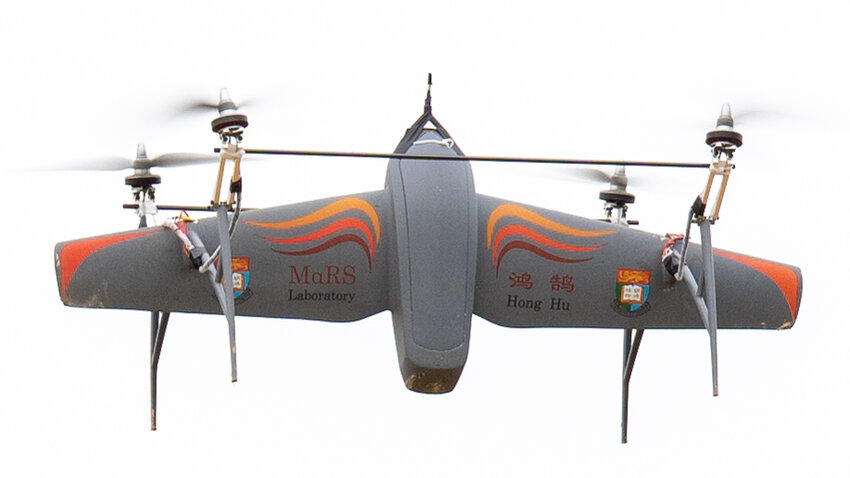
\includegraphics[width=0.4\textwidth]{Cap1/VTOL-TAIL.jpg}%
        \label{fig:vtol_a}%
    }
    \hfill
    \subfloat[Configuração tiltrotor.]{%
        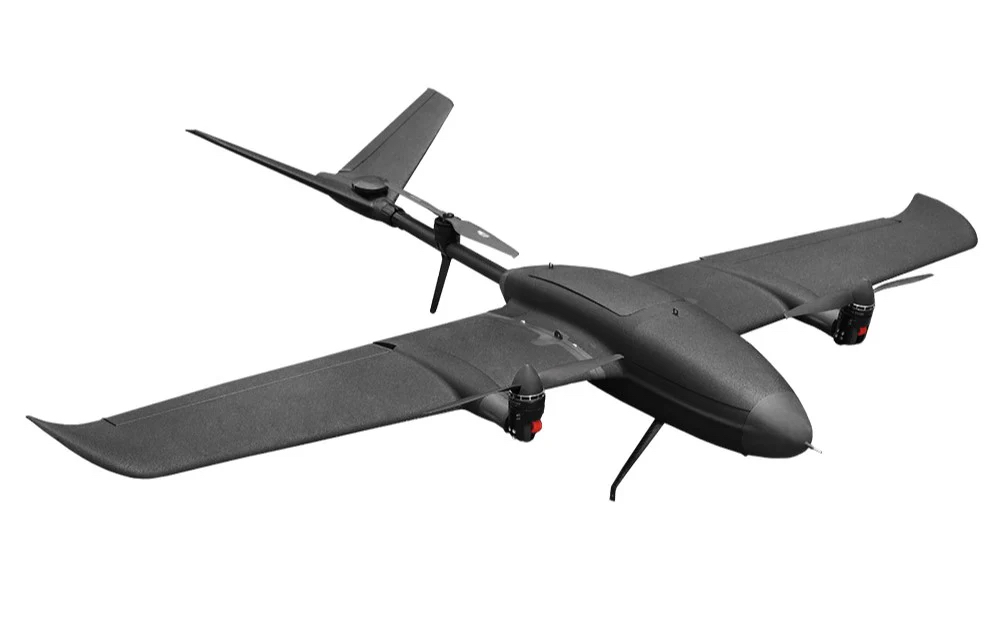
\includegraphics[width=0.4\textwidth]{Cap1/VTOL-TILT.jpg}%
        \label{fig:vtol_b}%
    }
    \\
    \subfloat[Configuração Híbrida.]{%
        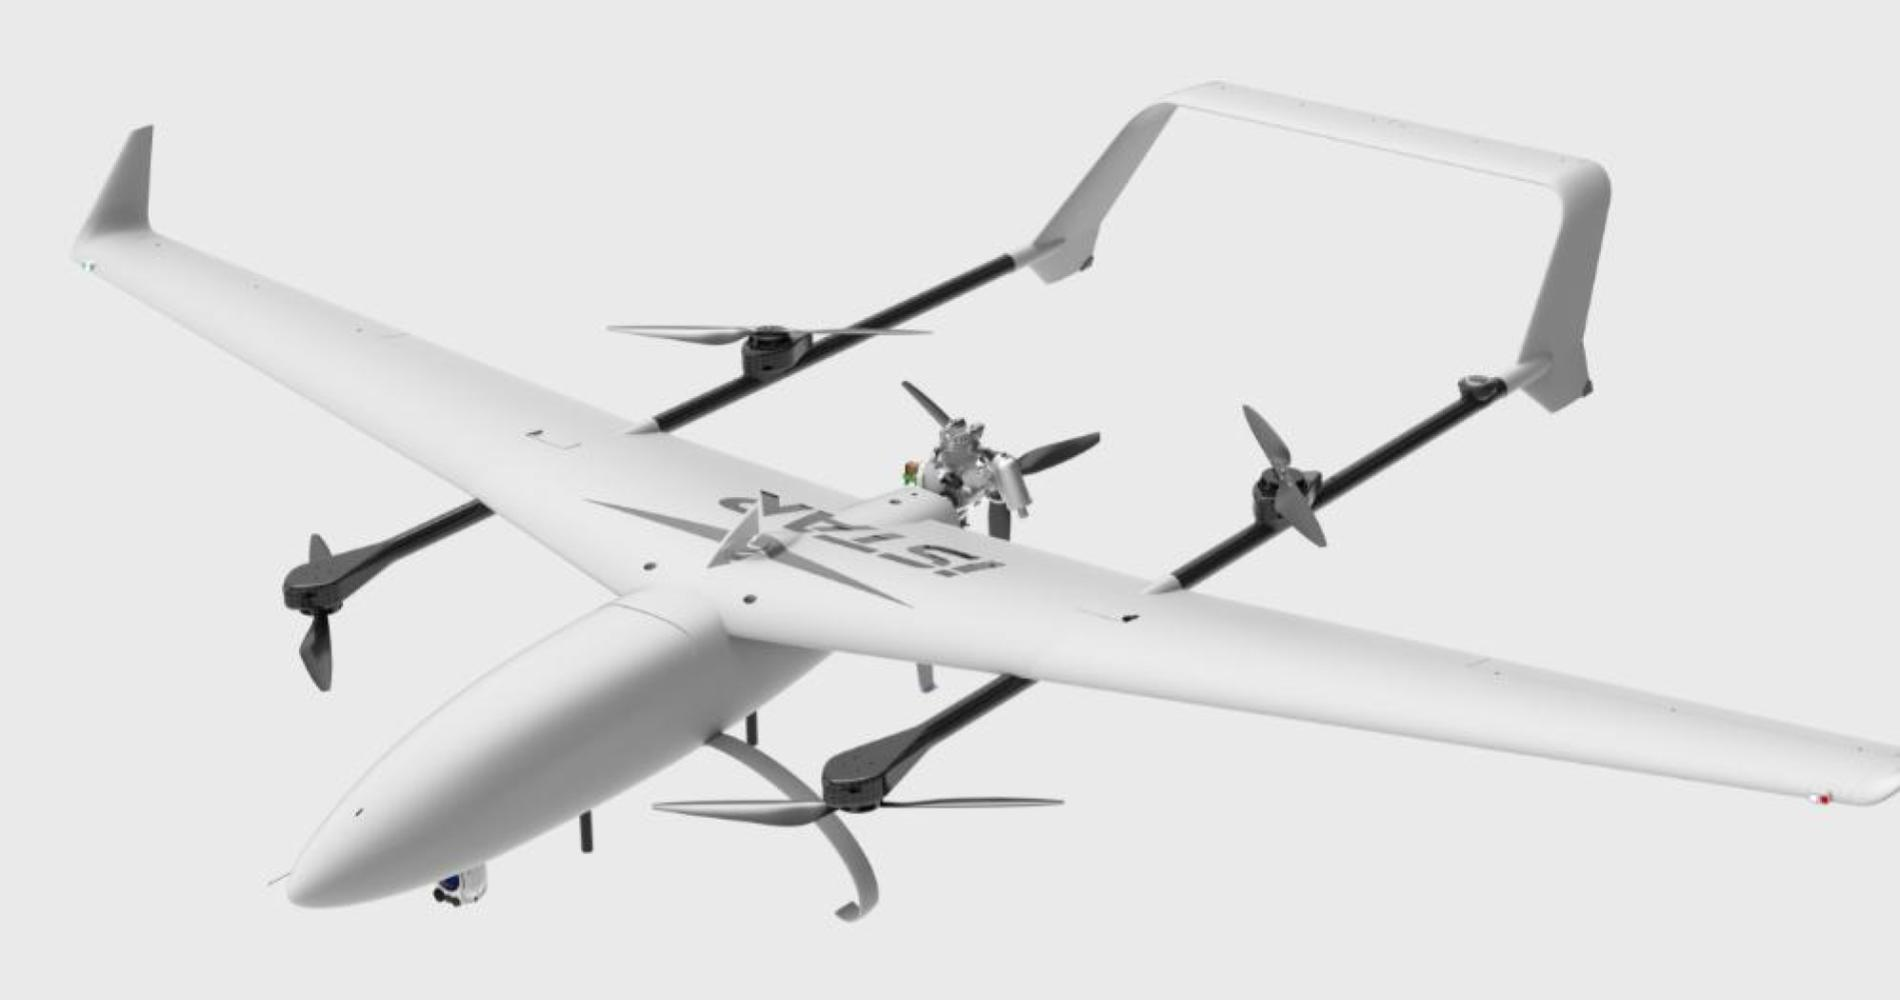
\includegraphics[width=0.4\textwidth]{Cap1/VTOL.jpg}%
        \label{fig:vtol_c}%
    }
    \caption{Configurações comuns de VTOL.}
    \label{fig:vtol_tipos}
\end{figure}

Apesar das vantagens físicas acumuladas dos dois modos, a complexidade dos modelos de representação desse sistema torna-se mais elevada, o que dificulta o projeto de controle, como apresenta \textcite{Graesdal2021}. Essa dificuldade decorre da união dos efeitos do modo multirrotor com a aerodinâmica do modo asa fixa, o que {\color{blue}dificulta} a separação da contribuição de cada um na avaliação das medidas dos sensores. O problema é mais evidente na {\color{blue}transição, fase em que as duas dinâmicas atuam de forma simultânea com magnitudes comparáveis, antes de a sustentação da asa se estabelecer e de os motores verticais serem desligados}.

Em projetos de multirrotores, é comum construir o modelo matemático apenas com os valores medidos da geometria da aeronave, com o peso e com experimentos de bancada dos motores. Nesse procedimento, o resultado é avaliado pela resposta do controlador projetado sobre um modelo não validado em dados reais, o que se mostra efetivo para essa classe de veículos \cite{Bouabdallah2007, Carino2015}. No caso do VTOL, entretanto, essa abordagem pode demandar esforço considerável, sem garantia de uma boa representação do sistema real{\color{blue}. Os ensaios de bancada caracterizam o empuxo e o torque dos rotores em ponto de operação fixo, e por isso não capturam os efeitos dinâmicos que surgem quando a aeronave se move, como os momentos de amortecimento gerados pela variação do empuxo de cada rotor com a rotação do corpo. Além disso, a estrutura de asa fixa desloca a distribuição de massa, introduzindo assimetrias de inércia ausentes nos quadrirrotores convencionais, e acrescenta superfícies que geram forças e momentos aerodinâmicos crescentes com a velocidade de translação.} Soma-se a isso a instabilidade do modo multirrotor, que inviabiliza a excitação do sistema em malha aberta, possível em algumas aeronaves de asa fixa, e dificulta a aplicação de métodos convencionais de identificação de sistemas \cite{Aguirre2015}.

{\color{blue}
Para situar a contribuição desta dissertação, buscou-se na literatura trabalhos dedicados à modelagem e à identificação de aeronaves VTOL híbridas, com atenção a três aspectos, o tratamento dado ao modo de voo pairado, a representação dos efeitos aerodinâmicos em baixa velocidade e a validação experimental dos modelos propostos. Três trabalhos recentes delimitam o estado atual dessa modelagem. O mais próximo desta dissertação é o trabalho de \textcite{Graesdal2021}, que estuda uma aeronave da mesma configuração híbrida e constrói o modelo completo a partir da formulação clássica de asa fixa, à qual acrescenta o empuxo e o contratorque dos multirrotores, obtendo as inércias de um modelo tridimensional detalhado da estrutura e os coeficientes aerodinâmicos iniciais do método de malha de vórtices, posteriormente refinados por identificação com dados de voo, pelo método do erro de saída, \gls{OEM}, nas dinâmicas longitudinal e látero-direcional. A validação experimental, contudo, restringe-se ao regime de asa fixa, em velocidades entre 17 e 22 m/s, enquanto o modo pairado não é ensaiado nem simulado, e a aerodinâmica é anulada abaixo de 1 m/s por um limiar arbitrário que contorna a indeterminação dos ângulos aerodinâmicos. O próprio autor reconhece como limitação que o modelo do modo multirrotor, restrito ao empuxo e ao contratorque, ainda precisa ser verificado com dados reais.

A transição entre os modos, por sua vez, é o foco de \textcite{Salahudden2023}, que a formula por meio de um coeficiente de mistura de variação contínua entre zero e um, responsável por suprimir os coeficientes aerodinâmicos em baixa velocidade até restarem apenas os efeitos dos rotores. O modelo serve de planta de simulação para estudos de controle que comparam configurações de três a oito rotores quanto ao consumo de potência e ao esforço de comando, de modo que o voo pairado é simulado apenas de forma implícita. As limitações são a ausência de validação experimental e a origem não declarada dos coeficientes aerodinâmicos, o que impede garantir que o modelo, a formulação ou os coeficientes representem uma aeronave real.

Entre os trabalhos levantados, o que trata o voo pairado com maior profundidade é o do grupo de pesquisa da NASA, no qual \textcite{Nguyen2025} deduzem analiticamente, pela teoria de elemento de pá, as derivadas de estabilidade e controle de um eVTOL de 3,8 toneladas nesse regime, contemplando o influxo induzido pela rotação do corpo, o momento de cubo, a força no plano do disco e os efeitos não estacionários. A dedução resulta em seis derivadas de momento, três de amortecimento associadas às taxas angulares e três associadas às velocidades lineares de translação, derivadas de estabilidade do voo pairado que os dois trabalhos anteriores não consideram em seus modelos. As contribuições aerodinâmicas da estrutura de asa fixa permanecem fora do escopo, por serem consideradas bem estabelecidas na literatura, e os coeficientes obtidos não são confrontados com dados de voo.

Em síntese, nenhuma das três referências identifica e valida experimentalmente o modelo do voo pairado: \textcite{Graesdal2021} o assume a partir da prática consolidada dos multirrotores, \textcite{Salahudden2023} apenas o simulam e \textcite{Nguyen2025} o deduzem analiticamente, sem confronto com dados de voo. Esta dissertação preenche essa lacuna ao identificar e validar, com dados de voos reais, o modelo do modo multirrotor em voo pairado.
}

{\color{blue}Para ocupar esse espaço,} esta dissertação parte de uma premissa consolidada na literatura de identificação de aeronaves: modelos estimados a partir de dados reais de voo representam a dinâmica do veículo com mais fidelidade do que os construídos apenas com medidas geométricas e ensaios de bancada \cite{Jategaonkar2015, Tischler2012}. Propõe-se aplicar métodos de identificação aos dados de voo do VTOL{\color{blue} em modo multirrotor, regime em que os efeitos dos rotores dominam e a contribuição da estrutura pode ser quantificada,} para obter um modelo matemático mais preciso e, com ele, um projeto de controle mais coerente e efetivo. Um modelo validado com critérios sólidos permite ainda simular os efeitos das entradas no sistema antes da implementação no protótipo físico. Essa simulação fornece uma melhor compreensão do comportamento do drone e de suas dinâmicas, aumentando a previsibilidade dos ensaios de voo.

Neste contexto, é necessária a utilização de técnicas específicas para a identificação de plantas instáveis, como as descritas por \textcite{Jategaonkar2015}. Convém ainda adotar uma metodologia que organize o processo completo, papel cumprido pela M4V, que vai do projeto das manobras de excitação à validação do modelo. Suas etapas intermediárias incluem o tratamento das medidas obtidas e a estimação de parâmetros com dados de voo, por métodos como o \gls{EEM} e o \gls{OEM}, avaliados segundo critérios quantitativos estabelecidos.

\section{Motivação}\label{sec:motivacao}
O desenvolvimento de sistemas de controle para aeronaves está diretamente associado à disponibilidade de um modelo matemático representativo de sua dinâmica. A partir de um modelo confiável é possível projetar e verificar controladores, estimar estados não medidos e simular o comportamento da aeronave antes dos ensaios em voo, reduzindo o número de campanhas experimentais necessárias \cite{Aguirre2015}. De fato, as estratégias de controle mais adequadas para quadrirrotores pressupõem o conhecimento prévio da dinâmica do sistema \cite{Quan2017}.

Na prática, porém, obter esse modelo para um \gls{VANT} de pequeno porte é uma etapa custosa e incerta. Uma alternativa comum é adotar um piloto automático de malhas pré-estabelecidas, isto é, um sistema embarcado cuja arquitetura de controle já vem definida pelo fabricante, organizada em malhas em cascata de posição, atitude e taxa angular, restando ao projetista apenas a sintonia experimental dos ganhos, como ocorre na controladora Pixhawk utilizada neste trabalho. Esse ajuste, contudo, exige extensas campanhas de voo, eleva os custos e impõe risco de acidentes, nem sempre com resultado satisfatório. Outra alternativa é construir o modelo apenas a partir da geometria, da massa e de ensaios de bancada dos motores, ou ainda adaptá-lo de modelos genéricos de aeronaves semelhantes. Essa via frequentemente não produz uma representação fiel, sobretudo no caso de um \gls{VTOL} híbrido, que combina os efeitos do modo multirrotor com a aerodinâmica do modo asa fixa e ainda não dispõe de modelos consolidados \cite{Saeed2018, Graesdal2021}.

Diante disso, a principal motivação deste trabalho é obter um modelo matemático representativo e validado do \gls{VTOL} em modo multirrotor por meio da identificação de sistemas a partir de dados reais de voo. Um modelo assim construído reduz a dependência de sucessivos ajustes empíricos, diminui o custo e o tempo de desenvolvimento, aumenta a previsibilidade dos ensaios e viabiliza tanto a simulação fiel da aeronave quanto o projeto de um controle de decolagem mais coerente e eficaz.

Cabe destacar que a metodologia de identificação empregada é consolidada na literatura aeronáutica, de modo que a contribuição deste trabalho não está em propor métodos novos. Ela reside na aplicação da cadeia completa, do dado bruto de voo ao controlador simulado, a uma classe de aeronave cuja modelagem permanece em aberto. A Figura \ref{fig:dh_foto} apresenta o protótipo \gls{DH}, que reúne uma asa fixa, quatro rotores dedicados ao voo vertical e um motor propulsor de cauda. Como se trata de uma plataforma particular, projetada por uma equipe de pesquisa do ITA, entrega-se o primeiro modelo identificado e validado do seu modo multirrotor, mais aderente aos dados de voo do que o obtido apenas com medidas geométricas e ensaios de bancada.

\begin{figure}[ht]
    \centering
    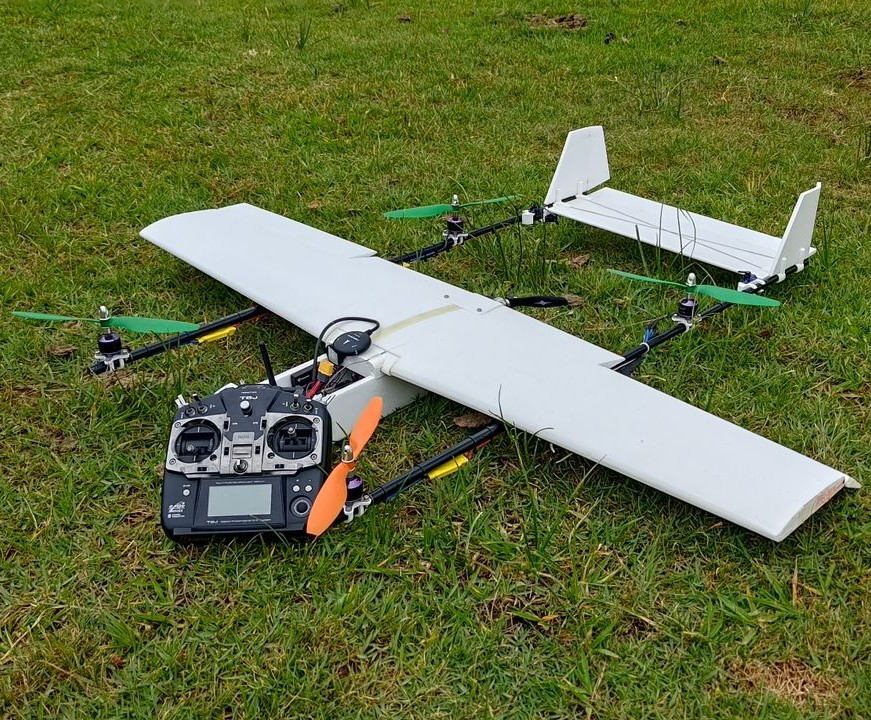
\includegraphics[width=0.5\textwidth]{Cap1/DH-REAL.jpeg}
    \caption{Fotografia do protótipo DH (Drone Híbrido).}
    \label{fig:dh_foto}
\end{figure}

\section{Objetivos}\label{sec:objetivos}
% GUIA — Objetivo geral (1 parágrafo):
%   . enuncie em uma frase: desenvolver/identificar um modelo matemático do VTOL
%     em modo multirrotor, a partir de dados de voo, para apoiar o controle de
%     decolagem
% >>> escreva aqui <<<

% GUIA — Abordagem (1 frase — opcional aqui):
%   . a identificação segue a metodologia no domínio do tempo de Jategaonkar:
%     EEM (estimativa inicial) -> OEM (refino por máxima verossimilhança)
%   % [ref] Jategaonkar
% >>> escreva aqui <<<

Este trabalho tem como objetivo geral identificar e validar um modelo matemático para a dinâmica de um drone VTOL, em configuração híbrida no modo multirrotor, através do uso de dados de logs de voo para treinamento e validação, além do desenvolvimento e da avaliação, em ambiente de simulação, de um projeto de controle de decolagem com PID em cascata. Para alcançar o objetivo geral, foram estabelecidos os seguintes objetivos específicos:

\begin{enumerate}
    \item \textbf{Modelagem matemática do drone em modo quadrirrotor}

    Desenvolver o modelo dinâmico do drone híbrido operando como quadrirrotor, tratando-o como um corpo rígido e isolando os efeitos aerodinâmicos do modo asa fixa. Esta etapa abrange as equações de movimento rotacional e translacional e o modelo do motor. A estrutura matemática resultante define os parâmetros que a identificação estima a partir dos dados de voo, combinação de estrutura teórica com estimação experimental que caracteriza a formulação de caixa cinza, adotada neste trabalho e formalizada no Capítulo~4. É esse único modelo, com estrutura teórica e parâmetros identificados experimentalmente, que serve de base para o projeto de controle.

    \item \textbf{Projeto de manobras e coleta dos dados de voo}

    Definir as manobras de excitação capazes de evidenciar a dinâmica de interesse e coletar os dados de voo de entrada e saída. A qualidade dos dados é determinante para a identificação, de modo que esta etapa garante a aquisição de sinais adequados ao processo de estimação.

    \item \textbf{Identificação do modelo a partir dos dados}

    Estimar os parâmetros do modelo no domínio do tempo, seguindo a metodologia M4V (\textit{Maneuvers, Measurements, Methods, Models and Validation}) e considerando a instabilidade do sistema. É nesta etapa que a estrutura teórica desenvolvida no primeiro objetivo recebe os parâmetros estimados a partir dos dados de voo. A ênfase recai sobre o método do erro de saída (\textit{Output-Error Method}, OEM), que simula o modelo e ajusta os parâmetros de forma iterativa, até minimizar a diferença entre a resposta simulada e as saídas medidas em voo. A estimativa inicial dessa otimização é fornecida pelo método do erro de equação (\textit{Equation-Error Method}, EEM).

    \item \textbf{Validação do modelo identificado}

    Verificar a coerência dos dados de entrada e avaliar a aderência do modelo identificado aos dados de voo reservados para validação, não utilizados na estimação. Para isso, simula-se a sua resposta aos comandos registrados nessas janelas e quantifica-se a concordância com as medições por meio de métricas estabelecidas, como o coeficiente de determinação ($R^2$) e o coeficiente de Theil (TIC), de forma a atestar a capacidade de representar a aeronave.

    \item \textbf{Projeto e simulação do controle}

    Projetar a malha de controle em arquitetura em cascata, com controladores PID para atitude, altitude e velocidade horizontal. Como o PID é uma técnica de controle linear e o modelo identificado é não linear, o projeto é realizado sobre a linearização desse modelo em torno do voo pairado, apresentada no Apêndice~\ref{ap:linearizacao}. A avaliação do desempenho é realizada exclusivamente por simulação, sem ensaios em voo do controlador. Para isso, a malha fechada é simulada nas plantas linear e não linear, e o contraste entre as respostas delimita a faixa de manobras em que a aproximação linear permanece representativa.
\end{enumerate}

    

% GUIA — Objetivos específicos (lista):
%   . quebre o objetivo geral em etapas (cada uma tende a virar um capítulo).
%     Ajuste à sua realidade; ponto de partida sugerido (descomente e edite):
% \begin{itemize}
%   \item levantar/definir o modelo dinâmico do VTOL em modo multirrotor;
%   \item projetar os experimentos e coletar os dados de voo;
%   \item estimar os parâmetros via EEM e refinar via OEM;
%   \item validar o modelo contra dados de voo não usados na identificação;
%   \item (se aplicável) avaliar o impacto no controle de decolagem.
% \end{itemize}

\section{Organização do trabalho}\label{sec:organizacao}
Esta dissertação está organizada em seis capítulos, descritos a seguir:

\begin{itemize}
    \item \textbf{Capítulo 1:} apresenta o contexto da dissertação, a motivação e os objetivos do projeto, delimitando o problema da modelagem do drone VTOL em modo multirrotor para o controle de decolagem.

    \item {\color{blue}\textbf{Capítulo 2:} descreve a plataforma física e a instrumentação do VTOL, a aeronave e sua geometria, o sistema de propulsão (motor e ESC) e a aviônica embarcada, e apresenta a metodologia de identificação: o problema da identificação de sistemas instáveis, as abordagens de caixa branca, cinza e preta e a identificação em malha fechada e aberta.}

    \item {\color{blue}\textbf{Capítulo 3:}} desenvolve a modelagem matemática da aeronave em modo quadrirrotor, abordando os sistemas e as transformações de coordenadas, as equações de movimento (modelos rotacional e translacional e a cinemática de Euler){\color{blue}, a composição das forças e momentos, as parcelas aerodinâmicas da estrutura} e o modelo do motor.

    \item \textbf{Capítulo 4:} apresenta a estratégia para a identificação do drone híbrido em modo quadrirrotor{\color{blue}, detalhando} as etapas da metodologia M4V adotada: a definição das manobras, a aquisição dos dados de saída{\color{blue}, com a campanha de voo realizada}, os métodos de estimação, com ênfase no OEM, o modelo não linear, os critérios de validação no domínio do tempo {\color{blue}e a verificação da coerência dos dados adquiridos}.

    \item \textbf{Capítulo 5:} avalia os resultados obtidos{\color{blue}: a} identificação do modelo não linear via OEM e {\color{blue}sua} validação. Com o modelo identificado, apresenta o projeto do controlador em cascata (arquitetura, controladores PID e ganhos), a simulação da malha fechada no modelo linear e a comparação do controle aplicado às plantas linear e não linear.

    \item \textbf{Capítulo 6:} apresenta as conclusões obtidas do trabalho desenvolvido e as sugestões de implementações para trabalhos futuros.
\end{itemize}

Complementarmente, o Apêndice~\ref{ap:bancada} reúne a caracterização experimental dos motores em bancada e o Apêndice~\ref{ap:linearizacao} apresenta a linearização do modelo em torno do voo pairado, que fundamenta o projeto de controle do Capítulo 5.
